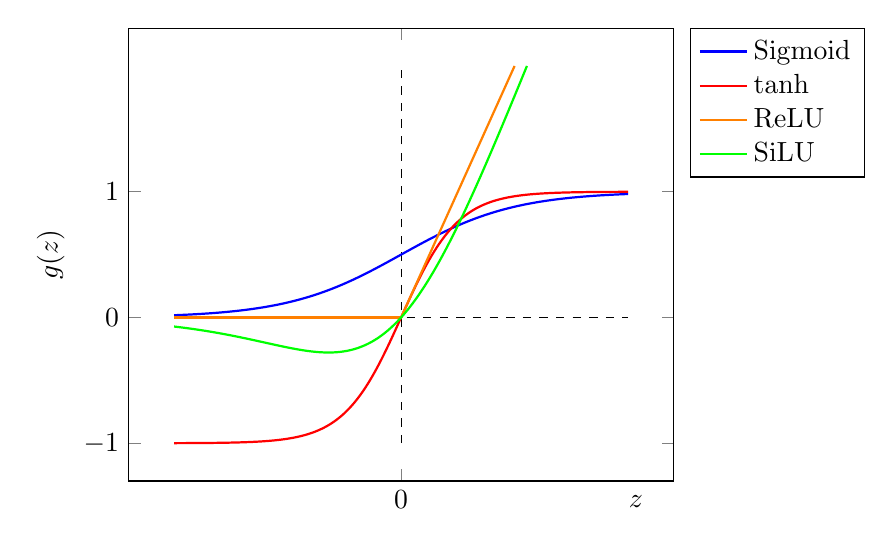
\begin{tikzpicture}
\pgfplotsset{width=8.5cm}
  \begin{axis}[
    domain=-4:4,
    xlabel=$z$,
    ylabel=$g(z)$,
    xtick={0},
    ytick={-1,0,1},
    every axis x label/.style={at={(0.9,-0.01)},anchor=north west},
    legend pos=outer north east,
    legend cell align=left
  ]
  % origin lines
  \addplot +[mark=none, black, dashed, forget plot] coordinates {(-4, 0) (4, 0)};
  \addplot +[mark=none, black, dashed, forget plot] coordinates {(0, -1) (0, 2)};

  % sigmoid 
  \addplot[thick, blue, samples=300] {1/(1+e^(-x))};%
  \addlegendentry{$\textnormal{Sigmoid}$}%

  % tanh
  \addplot[thick, red, samples=300] {tanh(x)};%
  \addlegendentry{$\textnormal{tanh}$}%
  
  % ELU
  %\addplot[thick, blue, samples=300, domain=-4:0, forget plot] {e^x - 1};%
  %\addplot[thick, blue, samples=300, domain=0:2] {x};%
  %\addlegendentry{$\textnormal{ELU}$}%

  % ReLU
  \addplot[thick, orange, samples=300, domain=-4:0, forget plot] {0};%
  \addplot[thick, orange, samples=300, domain=0:2] {x};%
  \addlegendentry{$\textnormal{ReLU}$}%

  % swish 
  % 1.278
  % 2.218
  \addplot[thick, green, samples=300, domain=-4:2.218] {x/(1+e^(-x))};%
  \addlegendentry{$\textnormal{SiLU}$}%

  \end{axis}%
\end{tikzpicture}